\chapter{System Analysis and Design}
This chapter details the analysis and design of the Verdant Search multimodal enterprise search engine, outlining its architecture, functional and non-functional requirements, and key design aspects based on Infinity Datatech's specific needs for optimizing enterprise knowledge management and document retrieval.

\section{Key System Modules}
The Verdant Search platform consists of five core modules, each providing distinct functionality while working together as an integrated system to address Infinity Datatech's multimodal search and retrieval needs.

\subsection{Module 1: User Management System}
This module handles authentication, authorization, and user profile management for the entire platform. It manages user login, registration, and session handling using secure authentication mechanisms including SSO integration with enterprise identity providers (LDAP, Okta, Azure AD). The role-based access control system assigns permissions ensuring users can only access documents they are authorized to view. The system maintains comprehensive audit trails of all access events, authentication attempts, and permission changes. Users can manage their profiles with configurable preferences including display settings, notification preferences, and search history management. The module also provides session management with automatic timeout and token validation to ensure secure access throughout the platform.

\subsection{Module 2: Search and Retrieval System}
This module forms the core functionality of Verdant Search, implementing hybrid search capabilities that combine BM25 keyword-based retrieval with HNSW vector search. The system accepts user queries through a text input interface, performing query normalization and sanitization. For keyword search, it utilizes an inverted index with BM25 scoring to enable fast lexical matching. Simultaneously, the vector search component encodes queries using Sentence-BERT embeddings and performs approximate nearest neighbor search using HNSW indices over CLIP-embedded documents and images. The system implements Reciprocal Rank Fusion (RRF) to combine scores from both retrieval methods, producing a unified ranked list. Advanced multimodal reranking is then applied to top candidates using BLIP-2 for cross-modal relevance scoring. The module supports metadata filtering, conversational search refinement, and maintains conversation context across multiple search turns through intelligent query rewriting.

\subsection{Module 3: Data Ingestion and Indexing System}
This module manages the complete data ingestion pipeline from multiple enterprise sources. It implements distributed crawling capabilities using Kafka for job coordination and task distribution across worker nodes. The system supports crawling from diverse sources including Confluence spaces (via REST API), Google Drive (via Drive API), Git repositories (via Git protocol), and local network shares (via SMB/NFS). Each crawler respects rate limits and implements exponential backoff for failed operations. Once documents are retrieved, the extraction subsystem processes them to extract both textual content and embedded images, with OCR support for scanned PDFs. The chunking component segments documents into semantic units using multiple strategies (heading structure, paragraph boundaries, fixed token counts) while maintaining overlap for context preservation. Finally, the indexing subsystem builds both inverted indices for BM25 using Pyserini and HNSW vector indices using FAISS, generating dense embeddings with Sentence-BERT for text and CLIP for images. The module supports both scheduled batch updates and real-time synchronization via webhooks.

\subsection{Module 4: Analytics and Monitoring System}
This module provides comprehensive observability into system performance and search quality. It collects and visualizes system metrics including query latency (p50, p95, p99), indexing throughput, and resource utilization using Prometheus and Grafana. The analytics engine tracks search quality metrics such as click-through rates, query success rates, and user engagement patterns. It monitors the health of all distributed components including crawler workers, indexing jobs, and retrieval services. The module generates alerts for anomalies in system behavior, performance degradation, or service failures, enabling proactive issue resolution. It also provides administrators with dashboards for monitoring indexing progress, query volume trends, and resource consumption across the platform.

\subsection{Module 5: RAG Generation System}
This module implements the retrieval-augmented generation capabilities that enable conversational interaction with search results. Upon receiving a user query, the system retrieves relevant document chunks using the Search and Retrieval module, then injects this context into carefully structured prompts for the LLM. The generation engine uses SGLang for efficient LLM serving, generating answers grounded exclusively in retrieved content to prevent hallucination. Answers are streamed to the user in real-time using server-sent events, formatted with markdown for readability. The system automatically adds inline citations linking to source documents with page numbers, enabling users to verify claims. The module maintains conversation history, detecting follow-up questions and rewriting them into standalone queries using the LLM with full conversational context. This creates a closed-loop system where LLM insights trigger new retrieval cycles, progressively refining search results. The module implements entailment checking to validate answer grounding and clearly indicates knowledge base limitations when queries cannot be answered from available documents.

\clearpage

\section{Hierarchical Task Analysis}

The Hierarchical Task Analysis (HTA) diagram shown in Figure \ref{fig:hta} illustrates the complete functional structure of the Verdant Search system. The system is organized into five primary modules: User Management, Search and Retrieval, Data Ingestion and Indexing, Analytics and Monitoring, and RAG Generation. Each module represents a distinct functional area that supports the overall system's purpose of providing comprehensive multimodal search, intelligent ranking, and conversational question answering capabilities for enterprise knowledge bases. The hierarchical breakdown shows how these primary tasks decompose into specific subtasks and operations, creating a clear visualization of the system's scope and organization. This task decomposition provides the foundation for the use cases and activity diagrams presented in subsequent sections.

\begin{figure}[H]
    \centering
    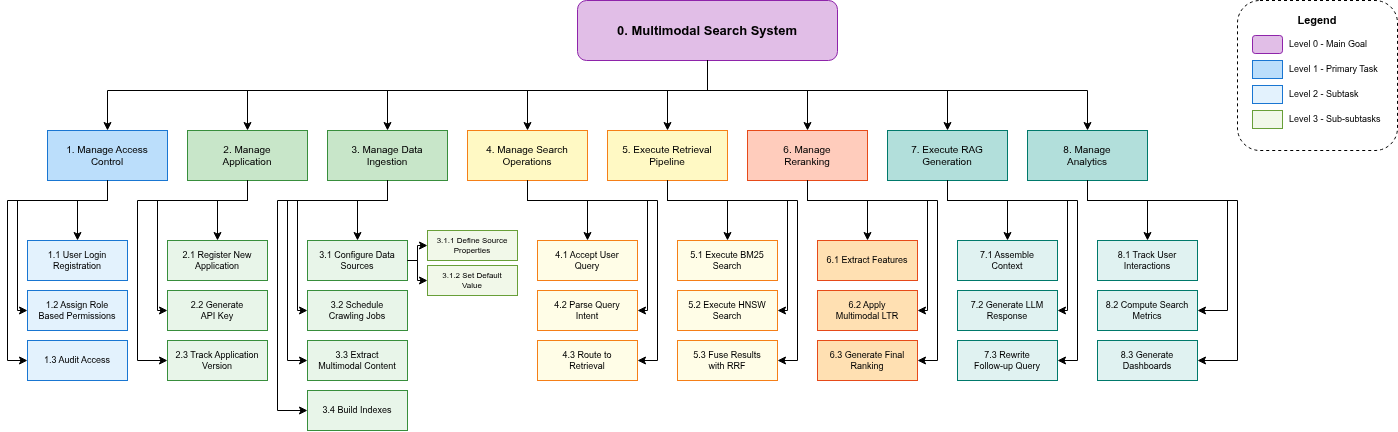
\includegraphics[width=\textwidth]{HTA.drawio.png}
    \caption{Hierarchical Task Analysis of Verdant Search System}
    \label{fig:hta}
\end{figure}
\clearpage


\section{Use Case Diagram}
\begin{figure}[H]
    \centering
    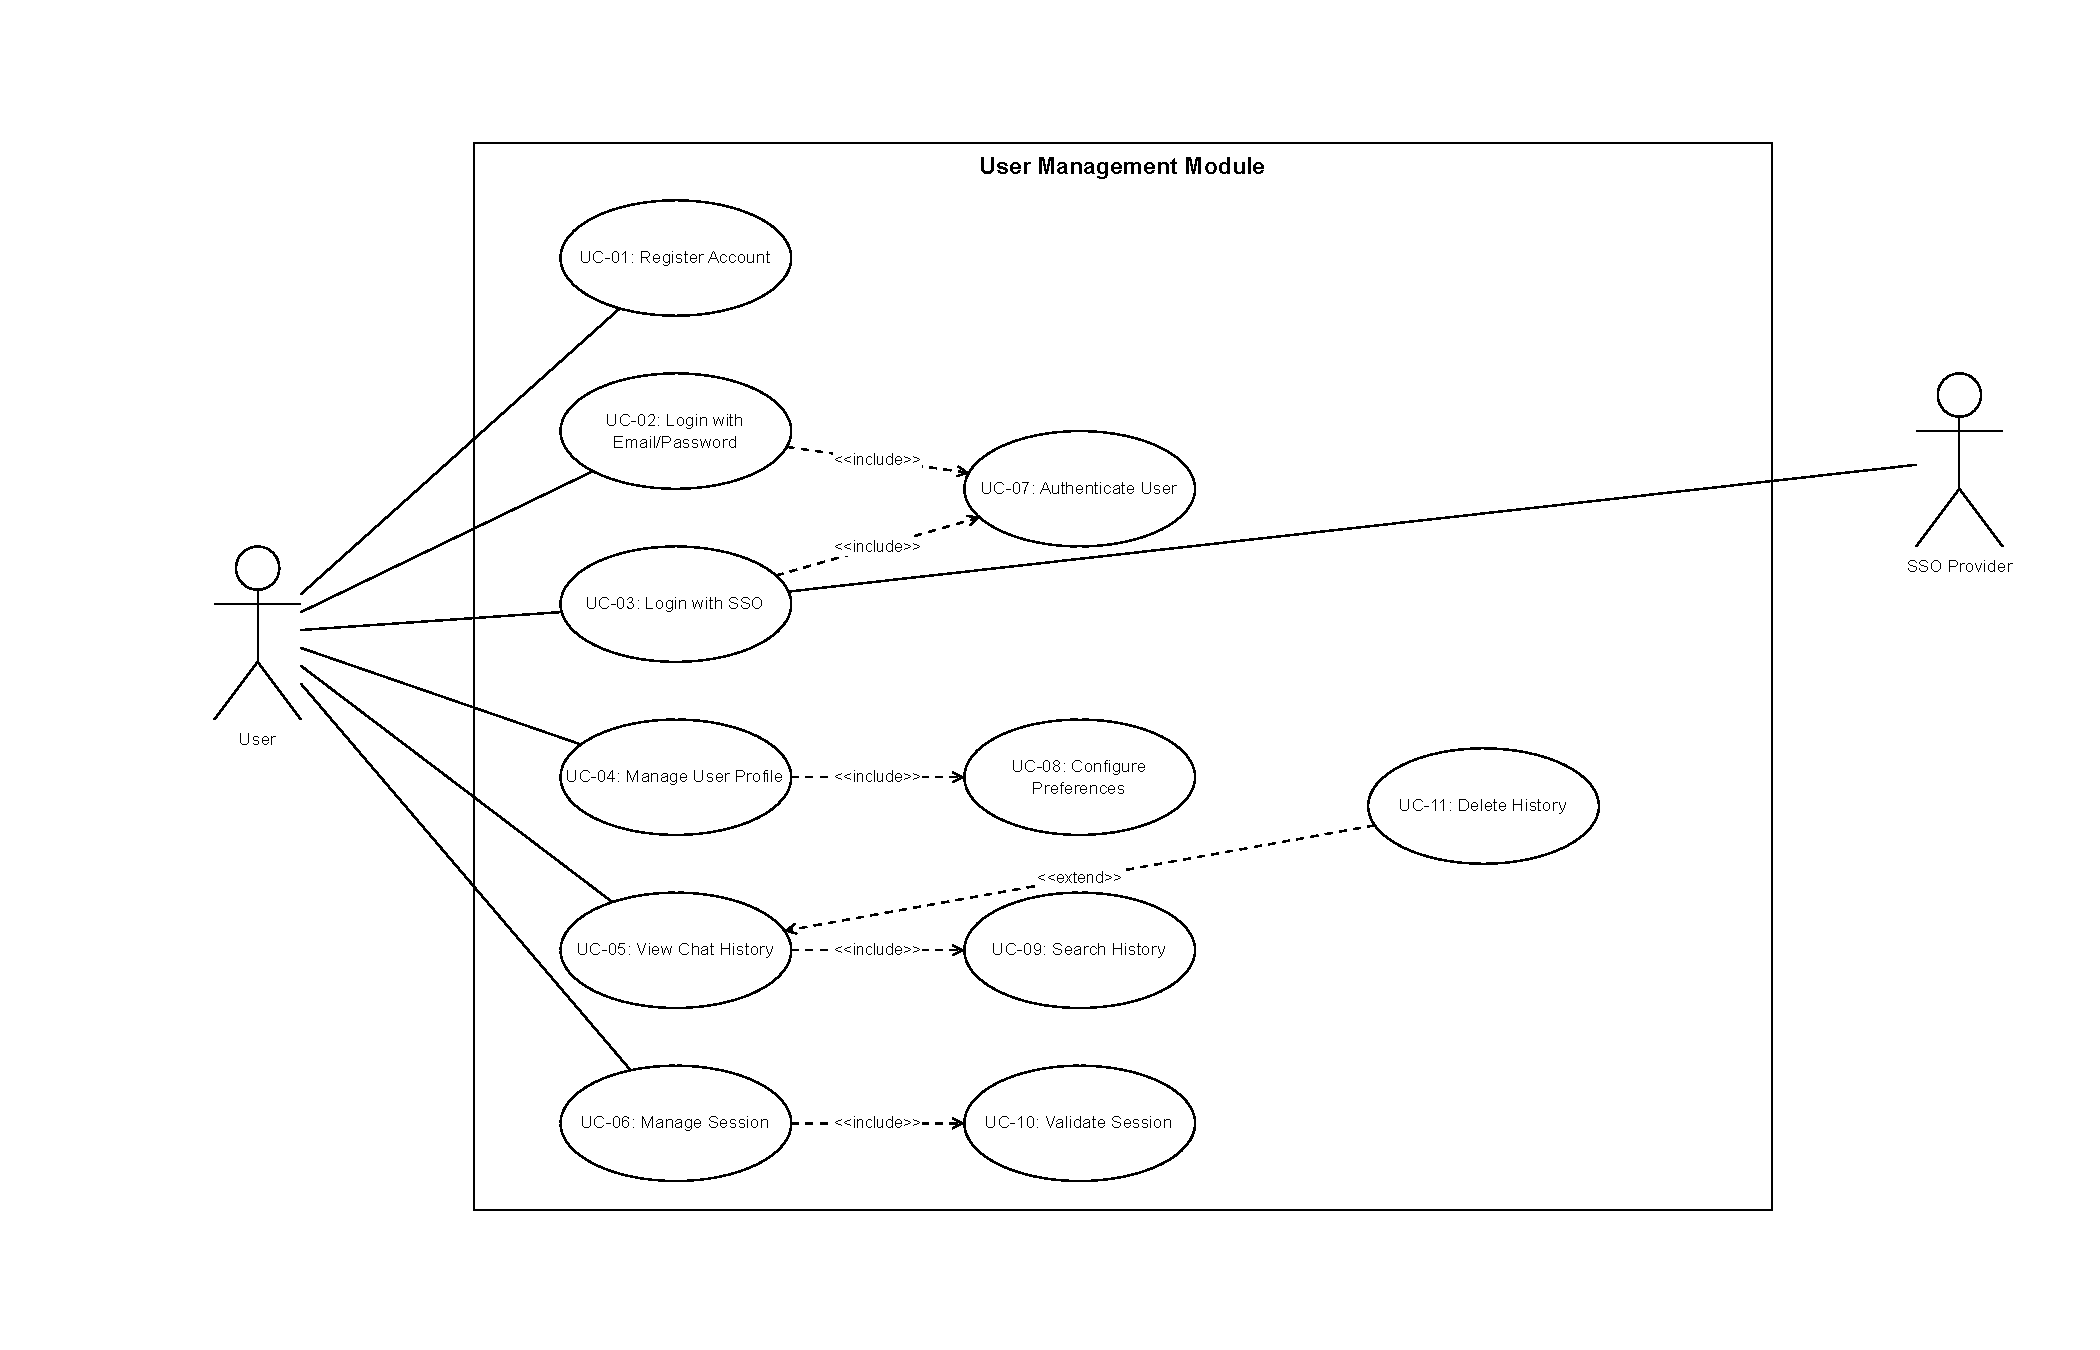
\includegraphics[width=0.95\textwidth,height=0.85\textheight,keepaspectratio]{updated_uc1.drawio.pdf}
    \caption{Use Case Diagram of Verdant Search System - User Management Module}
    \label{fig:usecase1}
\end{figure}

\noindent The Use Case Diagram illustrated above presents the User Management module of the Verdant Search system. This diagram shows how different actors (User, Administrator, System) interact with authentication, authorization, and profile management functionalities through various use cases.
\clearpage

\begin{figure}[H]
    \centering
    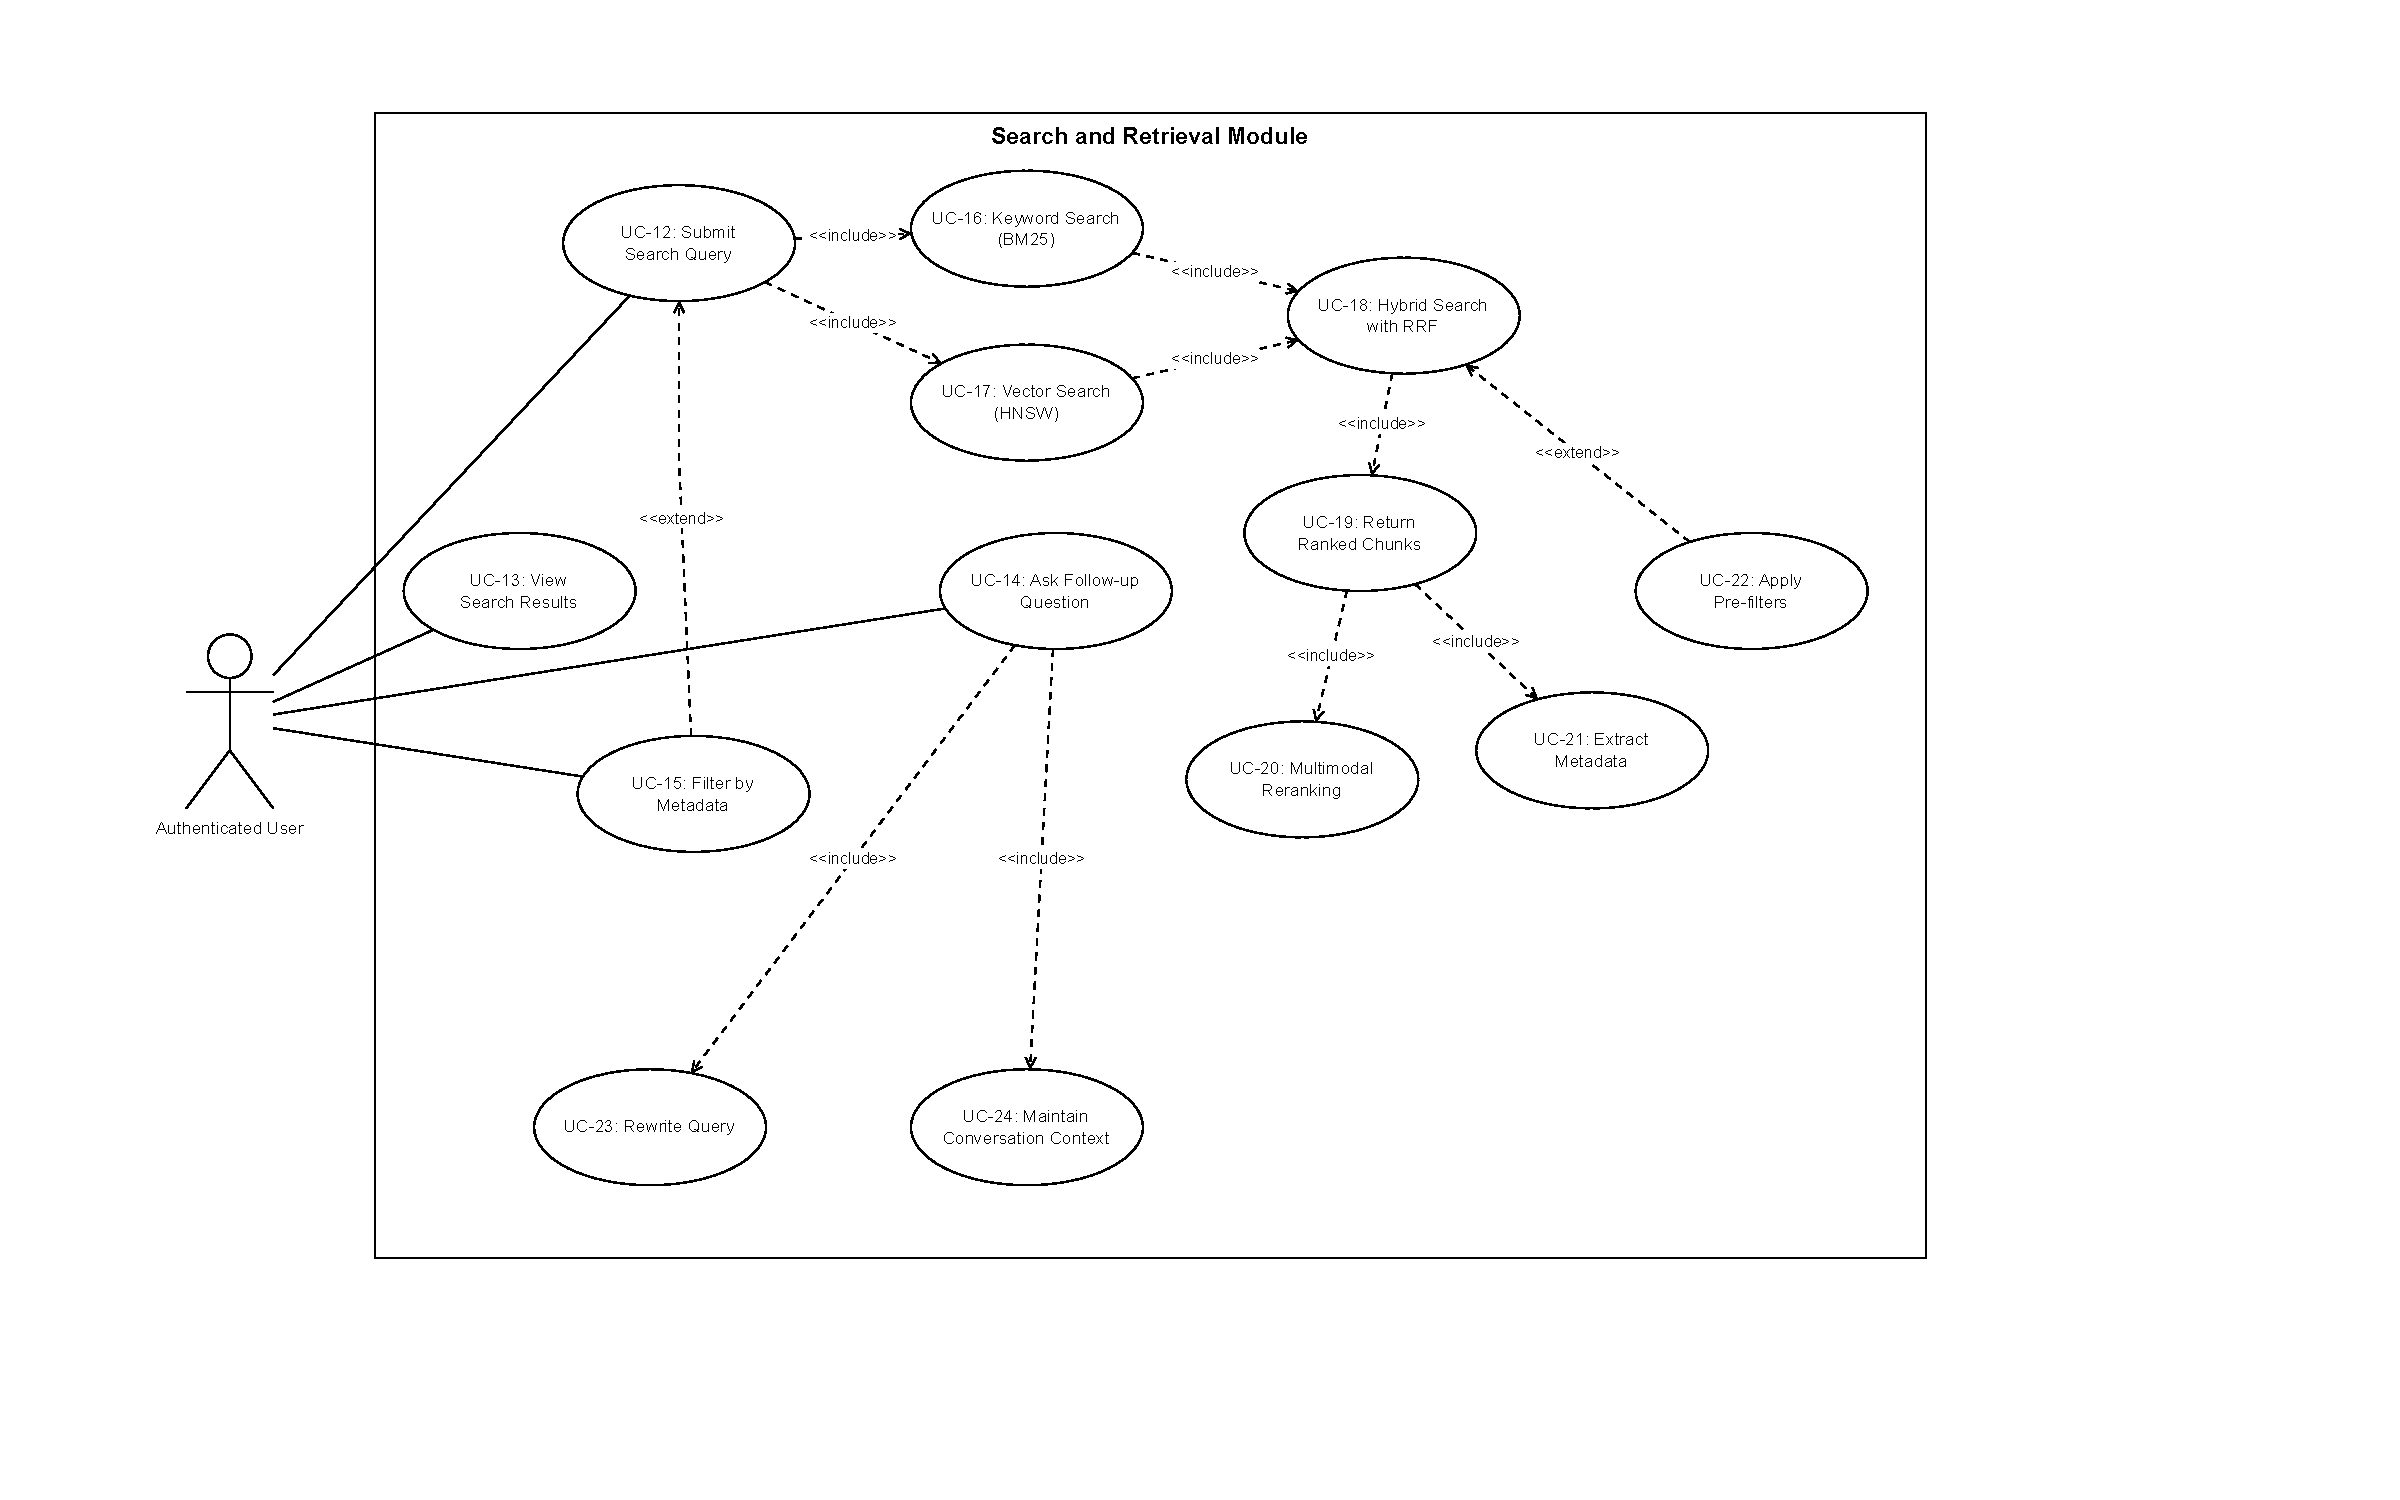
\includegraphics[width=0.95\textwidth,height=0.85\textheight,keepaspectratio]{updated_uc2.drawio.pdf}
    \caption{Use Case Diagram of Verdant Search System - Search and Retrieval Module}
    \label{fig:usecase2}
\end{figure}

\noindent This diagram presents the Search and Retrieval module, illustrating how users interact with the hybrid search system combining BM25 keyword search and HNSW vector search, along with multimodal reranking and conversational refinement capabilities.
\clearpage

\begin{figure}[H]
    \centering
    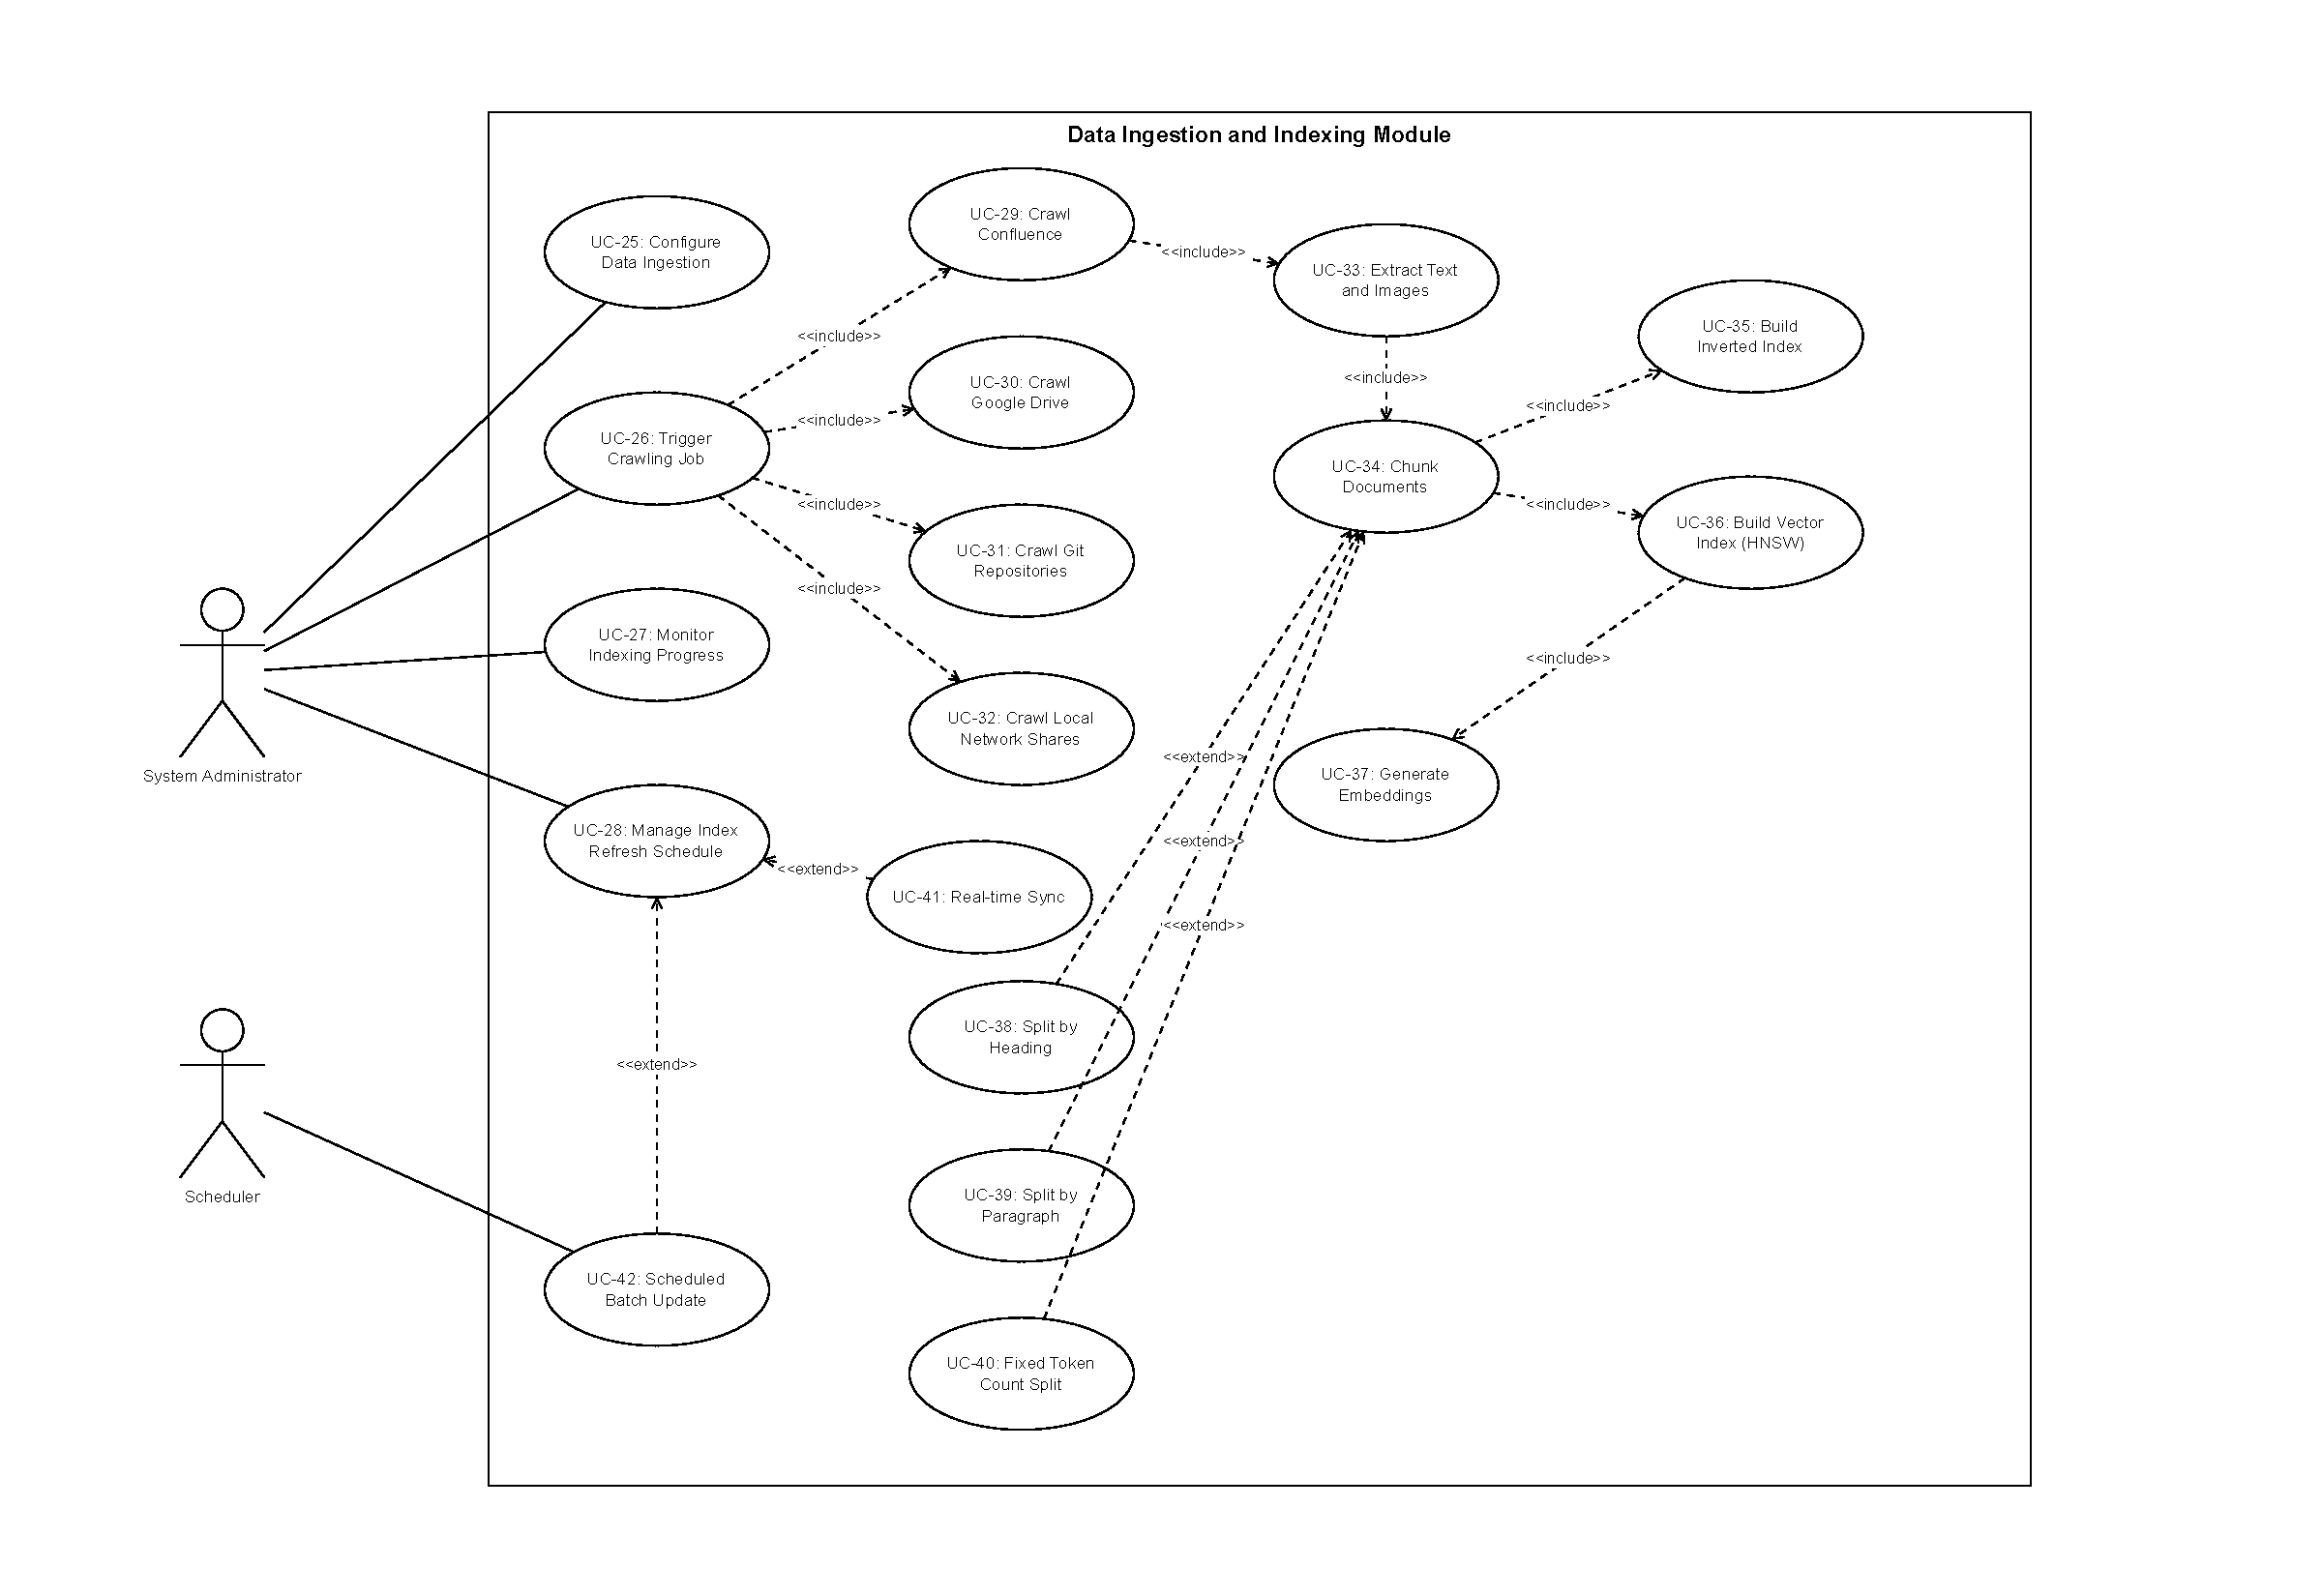
\includegraphics[width=0.95\textwidth,height=0.85\textheight,keepaspectratio]{updated_uc3.drawio.pdf}
    \caption{Use Case Diagram of Verdant Search System - Data Ingestion Module}
    \label{fig:usecase3}
\end{figure}

\noindent This diagram shows the Data Ingestion and Indexing module, depicting how administrators configure and manage distributed crawling across multiple enterprise data sources (Confluence, Google Drive, Git, network shares), and how the system processes, chunks, and indexes documents for efficient retrieval.
\clearpage

\begin{figure}[H]
    \centering
    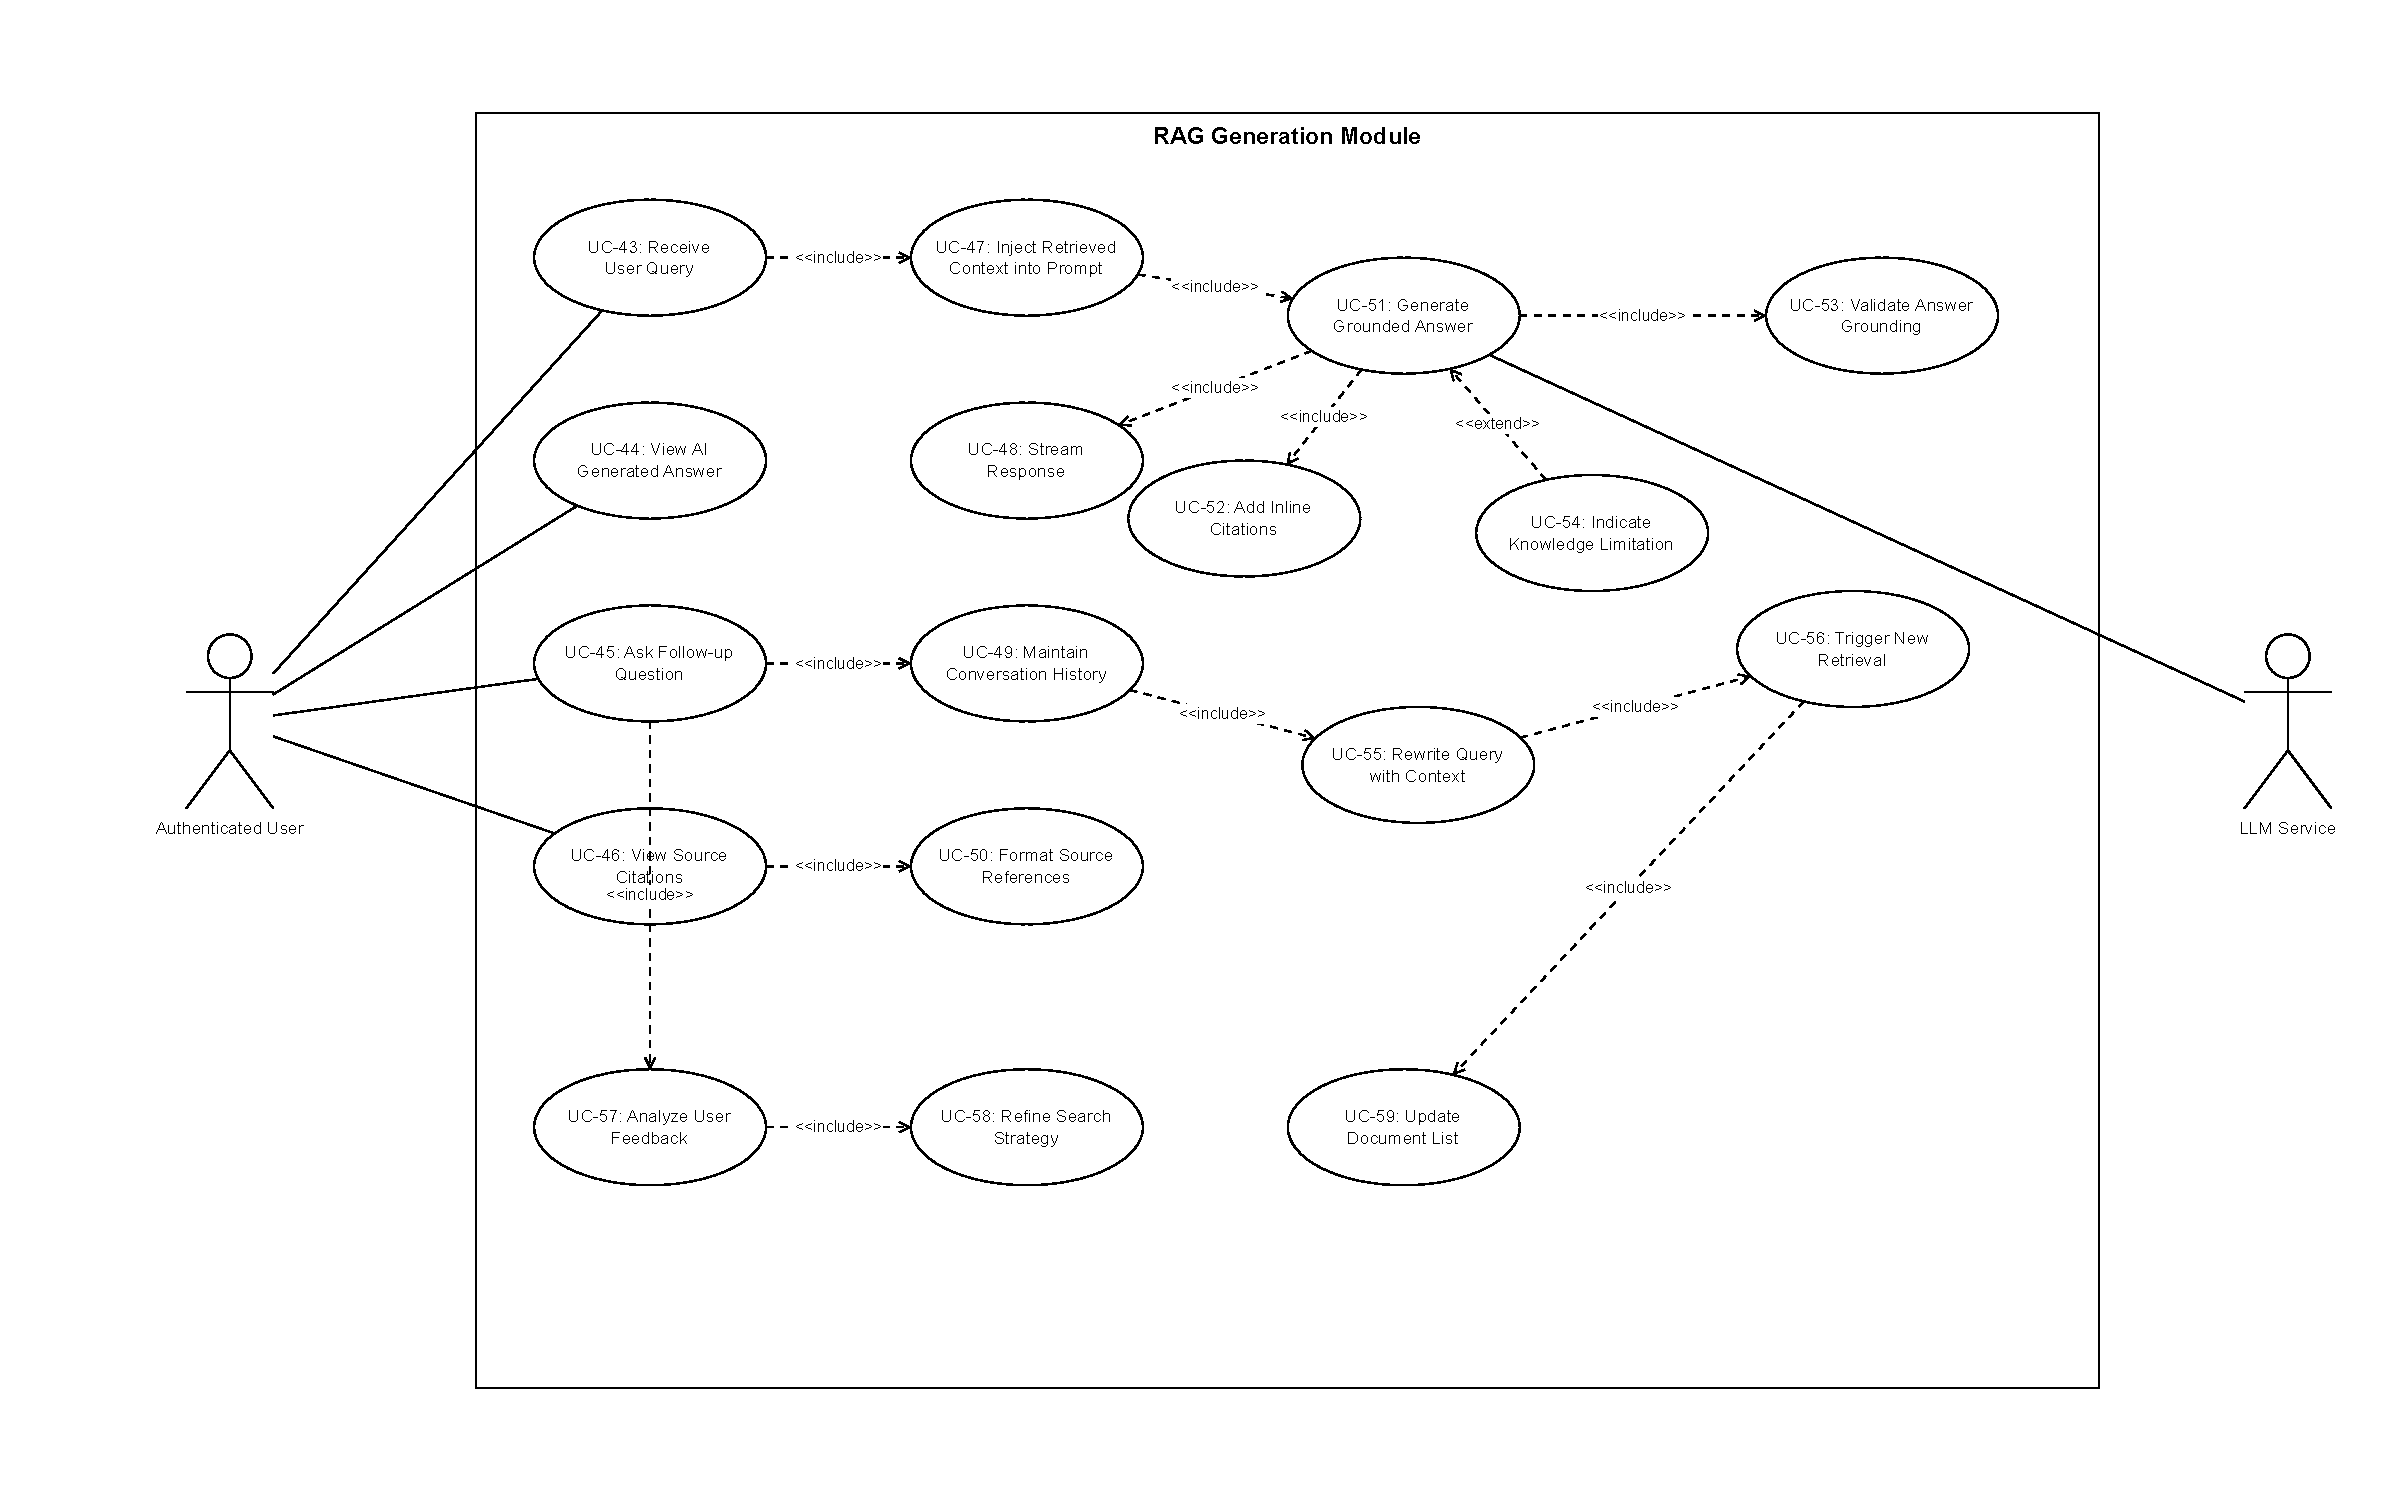
\includegraphics[width=0.95\textwidth,height=0.85\textheight,keepaspectratio]{updated_uc4.drawio.pdf}
    \caption{Use Case Diagram of Verdant Search System - RAG Generation Module}
    \label{fig:usecase4}
\end{figure}

\noindent This diagram illustrates the RAG Generation module, showing how the system generates AI-powered answers grounded in retrieved context, maintains conversational history, rewrites follow-up queries, and provides citations to source documents.
\clearpage


\section{Use Case Tables}

\begin{longtable}{|>{\raggedright\arraybackslash}p{0.08\textwidth}|>{\raggedright\arraybackslash}p{0.22\textwidth}|>{\raggedright\arraybackslash}p{0.62\textwidth}|}
\hline
\textbf{UC No.} & \textbf{Use Case Name} & \textbf{Functional Requirements (FRs)} \\
\hline
\endfirsthead

\hline
\textbf{UC No.} & \textbf{Use Case Name} & \textbf{Functional Requirements (FRs)} \\
\hline
\endhead

\hline \multicolumn{3}{r|}{{Continued on next page}} \\
\hline
\endfoot

\hline
\endlastfoot

% --- Module 1: User Management System ---
UC-1 & User Registration &
\begin{frequirements}
\item \textbf{FR-1.1:} The system shall allow a new user to register for an account by providing email and password.
\item \textbf{FR-1.2:} The system shall validate email format and enforce password strength requirements.
\item \textbf{FR-1.3:} The system shall send verification email upon successful registration.
\end{frequirements} \\
\hline

UC-2 & User Login via SSO &
\begin{frequirements}
\item \textbf{FR-1.4:} The system shall authenticate users via LDAP, Okta, or Azure AD SSO providers.
\item \textbf{FR-1.5:} The system shall support OAuth2 and SAML authentication protocols.
\item \textbf{FR-1.6:} The system shall generate JWT tokens for authenticated sessions.
\end{frequirements} \\
\hline

UC-3 & User Login via Email/Password &
\begin{frequirements}
\item \textbf{FR-1.7:} The system shall authenticate registered users based on email and password credentials.
\item \textbf{FR-1.8:} The system shall maintain user sessions after successful authentication.
\item \textbf{FR-1.9:} The system shall implement session timeout after 24 hours of inactivity.
\end{frequirements} \\
\hline

UC-4 & Manage User Profile &
\begin{frequirements}
\item \textbf{FR-1.10:} Users shall be able to update their display name, avatar, and notification preferences.
\item \textbf{FR-1.11:} Users shall be able to configure language and search result preferences.
\item \textbf{FR-1.12:} The system shall validate and store profile changes securely.
\end{frequirements} \\
\hline

UC-5 & View Chat History &
\begin{frequirements}
\item \textbf{FR-1.13:} The system shall display user chat history with timestamps and conversation summaries.
\item \textbf{FR-1.14:} Users shall be able to search within their chat history by keywords or date range.
\item \textbf{FR-1.15:} Users shall be able to export chat history in JSON or markdown format.
\end{frequirements} \\
\hline

UC-6 & Manage Session &
\begin{frequirements}
\item \textbf{FR-1.16:} The system shall validate session tokens on each authenticated request.
\item \textbf{FR-1.17:} The system shall automatically invalidate sessions after 24 hours.
\item \textbf{FR-1.18:} Users shall be able to manually log out to terminate their session.
\end{frequirements} \\
\hline

UC-7 & Authenticate User &
\begin{frequirements}
\item \textbf{FR-1.19:} The system shall verify user credentials against stored hashed passwords.
\item \textbf{FR-1.20:} The system shall log all authentication attempts with timestamps and outcomes.
\item \textbf{FR-1.21:} The system shall enforce rate limiting on failed authentication attempts.
\end{frequirements} \\
\hline

UC-8 & Configure User Settings &
\begin{frequirements}
\item \textbf{FR-1.22:} Users shall be able to set preferred search result display format.
\item \textbf{FR-1.23:} Users shall be able to configure notification preferences for search alerts.
\item \textbf{FR-1.24:} The system shall persist user settings across sessions.
\end{frequirements} \\
\hline

UC-9 & Search Chat History &
\begin{frequirements}
\item \textbf{FR-1.25:} The system shall support full-text search across user chat history.
\item \textbf{FR-1.26:} Search results shall highlight matching keywords in chat messages.
\item \textbf{FR-1.27:} The system shall rank search results by relevance and recency.
\end{frequirements} \\
\hline

UC-10 & Validate Session Token &
\begin{frequirements}
\item \textbf{FR-1.28:} The system shall verify JWT token signature and expiration on each request.
\item \textbf{FR-1.29:} The system shall reject expired or malformed tokens.
\item \textbf{FR-1.30:} The system shall return appropriate HTTP status codes for authentication failures.
\end{frequirements} \\
\hline

UC-11 & Delete Chat Entry &
\begin{frequirements}
\item \textbf{FR-1.31:} Users shall be able to delete individual chat conversations.
\item \textbf{FR-1.32:} Users shall be able to perform bulk deletion of chat history.
\item \textbf{FR-1.33:} The system shall prompt for confirmation before permanent deletion.
\end{frequirements} \\
\hline

% --- Module 2: Search and Retrieval System ---
UC-12 & Submit Search Query &
\begin{frequirements}
\item \textbf{FR-2.1:} The system shall accept search queries via text input interface.
\item \textbf{FR-2.2:} The system shall sanitize and normalize query text to prevent injection attacks.
\item \textbf{FR-2.3:} The system shall support query expansion with synonym detection.
\end{frequirements} \\
\hline

UC-13 & Display Search Results &
\begin{frequirements}
\item \textbf{FR-2.4:} The system shall present search results as a ranked list of documents.
\item \textbf{FR-2.5:} Each result shall display document title, snippet, and relevance score.
\item \textbf{FR-2.6:} The system shall highlight query keywords in document snippets.
\end{frequirements} \\
\hline

UC-14 & Ask Follow-up Question &
\begin{frequirements}
\item \textbf{FR-2.7:} Users shall be able to ask follow-up questions within the same conversation.
\item \textbf{FR-2.8:} The system shall detect whether input is a follow-up or new query.
\item \textbf{FR-2.9:} The system shall maintain conversation context across multiple turns.
\end{frequirements} \\
\hline

UC-15 & Filter Results by Metadata &
\begin{frequirements}
\item \textbf{FR-2.10:} Users shall be able to filter results by document type, date range, and source.
\item \textbf{FR-2.11:} The system shall apply filters before ranking to reduce computational cost.
\item \textbf{FR-2.12:} The system shall display active filters in the user interface.
\end{frequirements} \\
\hline

UC-16 & Perform Keyword Search &
\begin{frequirements}
\item \textbf{FR-2.13:} The system shall build and maintain an inverted index for BM25 retrieval.
\item \textbf{FR-2.14:} The system shall score documents using BM25 with tunable k1 and b parameters.
\item \textbf{FR-2.15:} The system shall return top K candidates from keyword search.
\end{frequirements} \\
\hline

UC-17 & Perform Vector Search &
\begin{frequirements}
\item \textbf{FR-2.16:} The system shall encode queries into dense vectors using Sentence-BERT.
\item \textbf{FR-2.17:} The system shall build HNSW index for approximate nearest neighbor search.
\item \textbf{FR-2.18:} The system shall return top K candidates from vector search with cosine similarity scores.
\end{frequirements} \\
\hline

UC-18 & Perform Hybrid Search &
\begin{frequirements}
\item \textbf{FR-2.19:} The system shall combine BM25 and vector search results using Reciprocal Rank Fusion.
\item \textbf{FR-2.20:} The system shall support weighted fusion with configurable alpha parameter.
\item \textbf{FR-2.21:} The system shall deduplicate results from both retrieval methods.
\end{frequirements} \\
\hline

UC-19 & Retrieve Context Chunks &
\begin{frequirements}
\item \textbf{FR-2.22:} The system shall return document chunks with surrounding context for RAG.
\item \textbf{FR-2.23:} Each chunk shall include metadata (filename, page number, timestamp).
\item \textbf{FR-2.24:} The system shall limit total context size to fit LLM context window.
\end{frequirements} \\
\hline

UC-20 & Apply Multimodal Reranking &
\begin{frequirements}
\item \textbf{FR-2.25:} The system shall apply multimodal reranking to top K candidates from hybrid search.
\item \textbf{FR-2.26:} The system shall use BLIP-2 vision-language model for cross-modal relevance scoring.
\item \textbf{FR-2.27:} The system shall reorder results based on multimodal relevance scores.
\end{frequirements} \\
\hline

UC-21 & Extract Chunk Metadata &
\begin{frequirements}
\item \textbf{FR-2.28:} The system shall attach source document filename to each chunk.
\item \textbf{FR-2.29:} The system shall include page number or section identifier for each chunk.
\item \textbf{FR-2.30:} The system shall record document creation and modification timestamps.
\end{frequirements} \\
\hline

UC-22 & Apply Pre-filtering &
\begin{frequirements}
\item \textbf{FR-2.31:} The system shall support filtering by document source before retrieval.
\item \textbf{FR-2.32:} The system shall enforce access control filters based on user permissions.
\item \textbf{FR-2.33:} The system shall apply date range filters if specified by user.
\end{frequirements} \\
\hline

UC-23 & Rewrite Follow-up Query &
\begin{frequirements}
\item \textbf{FR-2.34:} The system shall use LLM to rewrite follow-up questions into standalone queries.
\item \textbf{FR-2.35:} The system shall include conversation history as context for rewriting.
\item \textbf{FR-2.36:} The system shall trigger new retrieval cycle with rewritten query.
\end{frequirements} \\
\hline

UC-24 & Maintain Conversation Context &
\begin{frequirements}
\item \textbf{FR-2.37:} The system shall store conversation history in session memory.
\item \textbf{FR-2.38:} The system shall limit history to last 10 conversation turns to manage context size.
\item \textbf{FR-2.39:} The system shall provide conversation history to query rewriting module.
\end{frequirements} \\
\hline

% --- Module 3: Data Ingestion and Indexing System ---
UC-25 & Configure Data Sources &
\begin{frequirements}
\item \textbf{FR-3.1:} Administrators shall be able to configure Confluence, Google Drive, Git, and network share sources.
\item \textbf{FR-3.2:} The system shall validate source credentials and API permissions.
\item \textbf{FR-3.3:} The system shall encrypt and securely store source credentials.
\end{frequirements} \\
\hline

UC-26 & Trigger Distributed Crawling &
\begin{frequirements}
\item \textbf{FR-3.4:} Administrators shall be able to manually trigger crawling jobs.
\item \textbf{FR-3.5:} The system shall use Kafka for distributing crawl tasks across worker nodes.
\item \textbf{FR-3.6:} The system shall implement exponential backoff for failed crawl attempts.
\end{frequirements} \\
\hline

UC-27 & Monitor Indexing Progress &
\begin{frequirements}
\item \textbf{FR-3.7:} Administrators shall be able to view real-time indexing progress dashboard.
\item \textbf{FR-3.8:} The system shall display metrics including documents processed, errors, and throughput.
\item \textbf{FR-3.9:} The system shall provide estimated time to completion for indexing jobs.
\end{frequirements} \\
\hline

UC-28 & Manage Index Refresh &
\begin{frequirements}
\item \textbf{FR-3.10:} Administrators shall be able to schedule index refresh using cron expressions.
\item \textbf{FR-3.11:} The system shall support incremental index updates without full rebuilds.
\item \textbf{FR-3.12:} The system shall maintain index version history for rollback capability.
\end{frequirements} \\
\hline

UC-29 & Crawl Confluence &
\begin{frequirements}
\item \textbf{FR-3.13:} The system shall connect to Confluence instances via REST API.
\item \textbf{FR-3.14:} The system shall respect Confluence rate limits and implement pagination.
\item \textbf{FR-3.15:} The system shall extract page content, attachments, and comments.
\end{frequirements} \\
\hline

UC-30 & Crawl Google Drive &
\begin{frequirements}
\item \textbf{FR-3.16:} The system shall connect to Google Drive via Drive API with OAuth2 authentication.
\item \textbf{FR-3.17:} The system shall process Google Docs, Sheets, Slides, and PDF formats.
\item \textbf{FR-3.18:} The system shall extract sharing permissions and metadata from Drive files.
\end{frequirements} \\
\hline

UC-31 & Crawl Git Repositories &
\begin{frequirements}
\item \textbf{FR-3.19:} The system shall clone Git repositories using SSH or HTTPS protocols.
\item \textbf{FR-3.20:} The system shall index documentation files (Markdown, reStructuredText, text).
\item \textbf{FR-3.21:} The system shall associate commits with document versions for change tracking.
\end{frequirements} \\
\hline

UC-32 & Crawl Network Shares &
\begin{frequirements}
\item \textbf{FR-3.22:} The system shall access network shares via SMB and NFS protocols.
\item \textbf{FR-3.23:} The system shall authenticate using provided network credentials.
\item \textbf{FR-3.24:} The system shall recursively scan directory structures for documents.
\end{frequirements} \\
\hline

UC-33 & Extract Document Content &
\begin{frequirements}
\item \textbf{FR-3.25:} The system shall extract text from PDF, DOCX, PPTX, and HTML documents.
\item \textbf{FR-3.26:} The system shall extract embedded images with associated captions.
\item \textbf{FR-3.27:} The system shall apply OCR to scanned PDFs using Tesseract.
\end{frequirements} \\
\hline

UC-34 & Chunk Documents &
\begin{frequirements}
\item \textbf{FR-3.28:} The system shall segment documents into semantic chunks using heading structure.
\item \textbf{FR-3.29:} The system shall maintain 10\% chunk overlap to preserve context across boundaries.
\item \textbf{FR-3.30:} The system shall limit chunk size to 512 tokens for embedding model compatibility.
\end{frequirements} \\
\hline

UC-35 & Build Inverted Index &
\begin{frequirements}
\item \textbf{FR-3.31:} The system shall build inverted index using Pyserini framework.
\item \textbf{FR-3.32:} The system shall store term posting lists with term frequencies and positions.
\item \textbf{FR-3.33:} The system shall create index segments for incremental updates.
\end{frequirements} \\
\hline

UC-36 & Build HNSW Index &
\begin{frequirements}
\item \textbf{FR-3.34:} The system shall build HNSW graph index using FAISS library.
\item \textbf{FR-3.35:} The system shall configure M and ef\_construction parameters for index quality.
\item \textbf{FR-3.36:} The system shall persist HNSW index to disk for efficient loading.
\end{frequirements} \\
\hline

UC-37 & Generate Embeddings &
\begin{frequirements}
\item \textbf{FR-3.37:} The system shall generate text embeddings using Sentence-BERT model.
\item \textbf{FR-3.38:} The system shall generate image embeddings using CLIP vision encoder.
\item \textbf{FR-3.39:} The system shall batch embedding generation for GPU efficiency.
\end{frequirements} \\
\hline

UC-38 & Chunk by Heading &
\begin{frequirements}
\item \textbf{FR-3.40:} The system shall parse document structure to identify headings.
\item \textbf{FR-3.41:} The system shall create chunks at section boundaries defined by headings.
\item \textbf{FR-3.42:} The system shall preserve heading text as chunk metadata.
\end{frequirements} \\
\hline

UC-39 & Chunk by Paragraph &
\begin{frequirements}
\item \textbf{FR-3.43:} The system shall detect paragraph boundaries using newline patterns.
\item \textbf{FR-3.44:} The system shall merge small adjacent paragraphs to meet minimum chunk size.
\item \textbf{FR-3.45:} The system shall split large paragraphs at sentence boundaries.
\end{frequirements} \\
\hline

UC-40 & Chunk by Token Count &
\begin{frequirements}
\item \textbf{FR-3.46:} The system shall use tokenizer to measure chunk length in tokens.
\item \textbf{FR-3.47:} The system shall create fixed-size chunks of 512 tokens.
\item \textbf{FR-3.48:} The system shall implement sliding window with 10\% overlap.
\end{frequirements} \\
\hline

UC-41 & Sync with Webhooks &
\begin{frequirements}
\item \textbf{FR-3.49:} The system shall provide webhook endpoints for real-time update notifications.
\item \textbf{FR-3.50:} The system shall process webhook events to trigger incremental indexing.
\item \textbf{FR-3.51:} The system shall validate webhook signatures to prevent unauthorized updates.
\end{frequirements} \\
\hline

UC-42 & Schedule Batch Updates &
\begin{frequirements}
\item \textbf{FR-3.52:} Administrators shall be able to configure batch update schedules.
\item \textbf{FR-3.53:} The system shall execute scheduled crawls at specified intervals.
\item \textbf{FR-3.54:} The system shall send notification emails upon batch update completion.
\end{frequirements} \\
\hline

% --- Module 5: RAG Generation System ---
UC-43 & Receive User Query &
\begin{frequirements}
\item \textbf{FR-5.1:} The system shall accept user queries for RAG-based answer generation.
\item \textbf{FR-5.2:} The system shall validate query length and reject queries exceeding 1000 characters.
\item \textbf{FR-5.3:} The system shall queue queries during high load to prevent system overload.
\end{frequirements} \\
\hline

UC-44 & View Generated Answer &
\begin{frequirements}
\item \textbf{FR-5.4:} The system shall display AI-generated answers formatted with markdown.
\item \textbf{FR-5.5:} Answers shall include inline citations linking to source documents.
\item \textbf{FR-5.6:} The system shall highlight cited text when users click citation links.
\end{frequirements} \\
\hline

UC-45 & Ask Follow-up in RAG &
\begin{frequirements}
\item \textbf{FR-5.7:} Users shall be able to ask follow-up questions within RAG conversations.
\item \textbf{FR-5.8:} The system shall detect follow-up intent using conversation context.
\item \textbf{FR-5.9:} The system shall maintain both chat history and search result history.
\end{frequirements} \\
\hline

UC-46 & View Source Citations &
\begin{frequirements}
\item \textbf{FR-5.10:} Users shall be able to click citations to navigate to source documents.
\item \textbf{FR-5.11:} The system shall highlight cited passages in source document viewer.
\item \textbf{FR-5.12:} Citations shall display document title, page number, and relevance score.
\end{frequirements} \\
\hline

UC-47 & Inject Retrieved Context &
\begin{frequirements}
\item \textbf{FR-5.13:} The system shall inject top K retrieved chunks into LLM prompt.
\item \textbf{FR-5.14:} Context shall be formatted with clear delimiters and metadata.
\item \textbf{FR-5.15:} The system shall truncate context if it exceeds LLM context window limit.
\end{frequirements} \\
\hline

UC-48 & Stream LLM Response &
\begin{frequirements}
\item \textbf{FR-5.16:} The system shall stream LLM-generated text to users in real-time.
\item \textbf{FR-5.17:} The system shall use server-sent events (SSE) for streaming.
\item \textbf{FR-5.18:} The system shall handle connection interruptions gracefully.
\end{frequirements} \\
\hline

UC-49 & Maintain Conversation History &
\begin{frequirements}
\item \textbf{FR-5.19:} The system shall store conversation history in Redis cache.
\item \textbf{FR-5.20:} The system shall limit history to last 10 conversation turns.
\item \textbf{FR-5.21:} The system shall provide conversation history export functionality.
\end{frequirements} \\
\hline

UC-50 & Format Source References &
\begin{frequirements}
\item \textbf{FR-5.22:} The system shall format citations with document title, author, and timestamp.
\item \textbf{FR-5.23:} Citations shall use superscript numbering format [1], [2], etc.
\item \textbf{FR-5.24:} The system shall generate bibliography at end of answer listing all sources.
\end{frequirements} \\
\hline

UC-51 & Generate Grounded Answer &
\begin{frequirements}
\item \textbf{FR-5.25:} The LLM shall generate answers using only provided context chunks.
\item \textbf{FR-5.26:} The system shall instruct LLM to avoid hallucination in system prompt.
\item \textbf{FR-5.27:} The system shall mark uncertain responses with confidence qualifiers.
\end{frequirements} \\
\hline

UC-52 & Add Inline Citations &
\begin{frequirements}
\item \textbf{FR-5.28:} The system shall instruct LLM to include citation markers in generated text.
\item \textbf{FR-5.29:} Citations shall link to specific document chunks used for each claim.
\item \textbf{FR-5.30:} The system shall validate citation markers match provided sources.
\end{frequirements} \\
\hline

UC-53 & Validate Answer Grounding &
\begin{frequirements}
\item \textbf{FR-5.31:} The system shall use entailment model to verify answer claims against sources.
\item \textbf{FR-5.32:} The system shall flag unsupported claims for user review.
\item \textbf{FR-5.33:} The system shall log grounding validation scores for quality monitoring.
\end{frequirements} \\
\hline

UC-54 & Indicate Knowledge Gaps &
\begin{frequirements}
\item \textbf{FR-5.34:} The system shall detect when retrieved context is insufficient to answer query.
\item \textbf{FR-5.35:} The system shall display message indicating knowledge base limitations.
\item \textbf{FR-5.36:} The system shall suggest query refinements to improve retrieval.
\end{frequirements} \\
\hline

UC-55 & Rewrite Conversational Query &
\begin{frequirements}
\item \textbf{FR-5.37:} The system shall use LLM to rewrite follow-up questions into standalone queries.
\item \textbf{FR-5.38:} The system shall include full conversation history as rewriting context.
\item \textbf{FR-5.39:} The system shall preserve user intent while resolving coreferences.
\end{frequirements} \\
\hline

UC-56 & Trigger New Retrieval &
\begin{frequirements}
\item \textbf{FR-5.40:} The system shall automatically trigger search after query rewriting.
\item \textbf{FR-5.41:} The system shall use rewritten query for hybrid retrieval pipeline.
\item \textbf{FR-5.42:} The system shall cache rewritten queries to avoid duplicate processing.
\end{frequirements} \\
\hline

UC-57 & Analyze User Feedback &
\begin{frequirements}
\item \textbf{FR-5.43:} The system shall collect user ratings (thumbs up/down) for generated answers.
\item \textbf{FR-5.44:} The system shall store feedback with associated queries and contexts.
\item \textbf{FR-5.45:} The system shall analyze feedback patterns to identify quality issues.
\end{frequirements} \\
\hline

UC-58 & Refine Search Strategy &
\begin{frequirements}
\item \textbf{FR-5.46:} The system shall adjust retrieval parameters based on feedback analysis.
\item \textbf{FR-5.47:} The system shall increase diversity when users repeatedly refine queries.
\item \textbf{FR-5.48:} The system shall log strategy adjustments for performance evaluation.
\end{frequirements} \\
\hline

UC-59 & Update Document List &
\begin{frequirements}
\item \textbf{FR-5.49:} The system shall refresh displayed document list after new retrieval.
\item \textbf{FR-5.50:} Updated list shall maintain scroll position from previous view.
\item \textbf{FR-5.51:} The system shall highlight newly added documents from refined search.
\end{frequirements} \\
\hline

\end{longtable}
